\begin{frame}
\frametitle{Problem Statement-Triangle Construction}
\begin{enumerate}[label=(\roman*)]
\item Construct $\triangle LMN$ right angled at M such that LN $=$ 5  MN $=$ 3\\

\textbf{Soln:}\\
\url{https://github.com/Rajolep/_Geometry/blob/master/codes/triangle/draw_triangle.py}
\url{https://github.com/Rajolep/_Geometry/blob/master/figs/construc.tex}
\begin{figure}
\begin{tikzpicture}
[scale =0.7,>=stealth,point/.style = {draw, circle, fill = black, inner sep = 1pt},]
\node (L) at (0,4)[point,label=above :$L$] {};
\node (M) at (0,0)[point,label=below :$M$] {};
\node (N) at (3,0)[point,label=below :$N$] {};

\draw (L)--(M);
\draw (M)--(N);
\draw (L)--(N);

\tkzMarkRightAngle[draw=red,size=.2](L,M,N)
 
\end{tikzpicture}
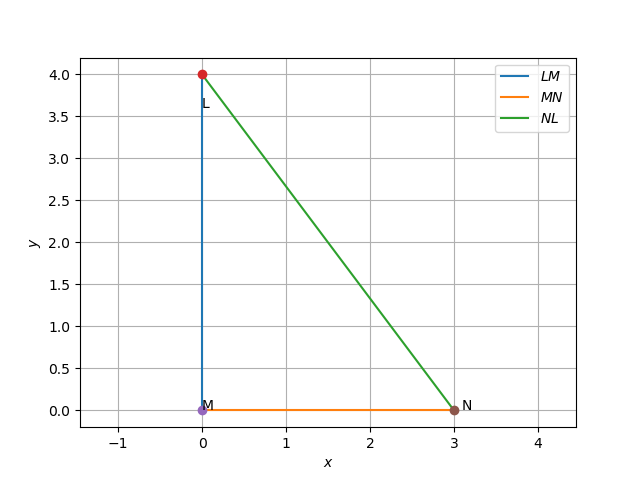
\includegraphics[scale=0.2]{./figs/tricon.png}
\end{figure}
\end{enumerate}
\end{frame}